\section{User Trust}
    Due to wide interest spanning many disciplines it is difficult, if not impossible, to write a succinct definition of trust that would appease all interested parties. However the following definition adapted from \cite{Harrison_McKnight2004-vv} is broad enough to avoid too much contention:

    \begin{description}
        \item [Trust:] to willingly and securely become vulnerable, or depend on, a trustee (e.g., another person, institution, or an AIA) having taken into consideration the characteristics (e.g., benevolence,  integrity,  competence)  of  the  trustee.
    \end{description}

    If you are going to give feedback to a user, you have to know what drive the decision making process of the agent.

    Trust is critical in interpersonal relationships, and it affects the dynamics of systems as simple as interpersonal relationships to more complicated ones such as financial markets and governments \cite{Fukuyama1995-un}. Consequently, researchers in psychology, sociology, and economics have historically sought to understand the fundamental principles of trust, each with the aim of understanding their field better \cite{Gambetta1988-pi}. Moral philosophers have also thought intently about the topic \cite{Baier1986-im}.

    In work relating to business management \cite{D_Harrison_Mcknight1996-ng,McKnight1998-ty} performed what is, to my knowledge, the first multi-disciplinary survey  and unification of trust literature, and condensed it into a single typology. That model is shown, with some minor adaptations, in Figure \ref{202769}. Notice that the three main dimensions --- Dispositional Trust, Institutional Trust, and Interpersonal Trust --- are connected in such a way as to indicate some causal relationships between them.

    **Each of the three main categories are made up of sub-categories. Figure XXXX shows the breakdown. Add more here**

    Trust is generally understood to exist between people. Is it possible for a human to enter into a trusting relationship with an AIA? In their paper regarding important human factors that should be considered when designing autonomous machines \cite{Sheridan1984-kx} are seemingly the first to discuss the idea that trust relationships between humans and autonomous systems are important, and to suggest that humans need some assurance that the "commands will be carried out properly". They also mention the idea that "there needs to be an accurate perception of [the autonomous system's] trustworthiness". Finally they suggest that "appropriate criteria for trust need to be studied to develop a theory of trust in supervisory control".

    A few years later \cite{Muir1987-mk} and later in more detail \cite{Muir1994-ow}, create a psychologically based model of trust that considered the "component expectations of trust" of \cite{Barber1983-yc} and the dynamic evolution of trust from \cite{Rempel1985-sg}, to make a framework for studying trust in human-machine relationships.

    That humans actually do feel trust towards machines has been experimentally confirmed several times in research using common subjective psychological questionairres. See \cite{Muir1996-gt,Reeves1997-ad,Groom2007-bz,Mcknight2011-gv,Riley1996-qm,Bainbridge2011-pl,Kaniarasu2012-mo,Salem2015-md,Desai2012-rc, Freedy2007-sg, Wang2016-id, Inagaki1998-cl, Kaniarasu2013-ho} for some examples.

    Many would not be surprised to know that trust is critical in interpersonal relationships, and that it affects the dynamics of systems as simple as interpersonal relationships to more complicated ones such as financial markets \cite{Fukuyama1995-un} and governments. Consequently, researchers in psychology, sociology, and economics have historically sought to understand the fundamental principles of trust, each with the aim of understanding their field better \cite{Gambetta1988-pi}. Moral philosophers have also thought intently about the topic \cite{Baier1986-im}.

    In the early days of the internet there was a surge of interest in trust due to the appearance of e-commerce. Suddenly, a new forum for buying and selling wares and services appeared. How could relationships of trust be built between consumers and vendors in a new `online' ecosystem? Many researchers focused their efforts on exploring how to establish an ecosystem that would nurture the growth and prosperity of online businesses \cite{McKnight2001-fa}. This research is useful to those seeking to understand trust today because it focused on building such an ecosystem. Consequently the more practical understanding emerged that included some thoughts about how to affect trust. This survey will not exhaustively review the literature on trust; those interested might refer to the following works by \citet{McKnight2001-fa}, and \citet{Lewicki2006-hj}.

    Due to wide interest spanning many disciplines it is difficult, if not impossible, to write a succinct definition that would appease all interested parties. In their work relating to e-commerce \citet{McKnight2001-fa} reviewed much of the existing trust literature and attempted to distill the main concepts into a trust model that spanned disciplines. That model is shown, with some minor adaptations, in Figure \ref{fig:UserTrust}. Notice that the three main dimensions --- Dispositional Trust, Institutional Trust, and Interpersonal Trust --- are connected in such a way as to indicate some causal relationships between them. As trust cannot be directly measured there is no existing method with which to quantify the more detailed relationships between each of the dimensions of trust.

	\begin{figure}[htbp]
    	\centering
     	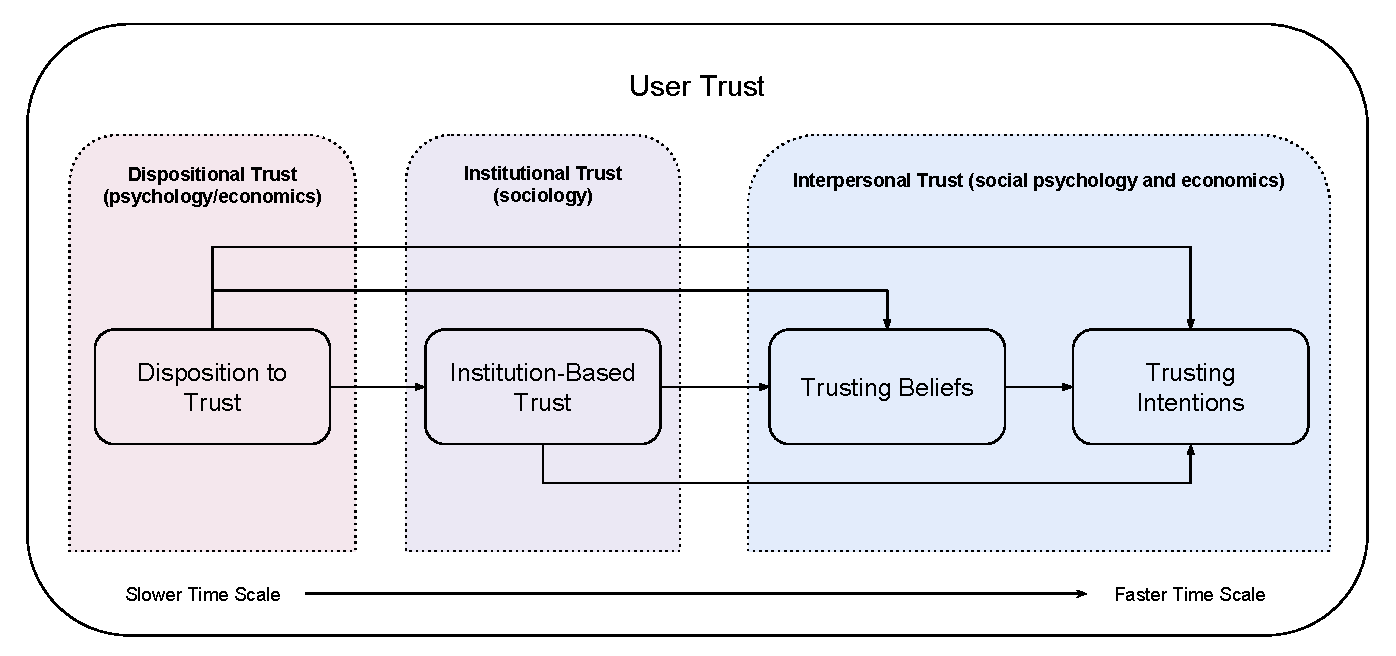
\includegraphics[width=0.9\textwidth]{Figures/UserTrust}
    	\caption{Interdisciplinary trust model proposed by \citet{McKnight2001-fa}. The three main categories are delineated and corresponding disciplines that are interested are listed within parentheses.}
        \label{fig:UserTrust}
    \end{figure}

    Something that is well accepted among researchers of all discplines is that trust results in some kind of behavior or action, which \citet{McKnight2001-fa} calls `trust-related behaviors' (TRBs). In the case of a human-autonomy relationship examples of TRBs might be the kinds of tasks the human user assigns to the autonomy, or whether the human will use a plan produced by the autonomy.

    \subsection{Distrust}
        As reviewed and discussed in \cite{Lewicki1998-ox}, and formalized in \cite{McKnight2001-gz} low trust is not the same as distrust, neither is low distrust the same as trust. \citet{McKnight2001-gz} suggest that "the emotional intensity of distrust distinguishes it from trust". They explain that distrust comes from emotions like: wariness, caution, and fear. Whereas, trust stems from emotions like: hope, safety, and confidence. Trust and distrust are orthogonal elements that define a person's trust-related behavior towards a trustee. \citet{Lewicki1998-ox} list several behaviors that stem from different combinations of trust and distrust; these are shown in Figure \ref{423053}.

        In \cite{Harrison_McKnight2001-hm} models for trust and distrust are proposed, and in later studies empirical evidence to validate some of the dimensions of both models was performed. \citet{McKnight2002-qx} is an empirical study that validates the model and quantifies the relationships between the model dimensions, and \cite{Harrison_McKnight2004-vv} investigates and quantifies the relationship between dispositional distrust and web-site usage. Finally, \cite{McKnight2006-ce} revisits the position of \cite{McKnight1998-ty} and concludes that research had largely confirmed the model.

        In this paper on the trust axis will be explicitly considered. Distrust has been shown to vary with perceived risk \cite{Harrison_McKnight2004}. Because of this it is not too much of a stretch to treat it as constant when dealing with a user in a situation where risk is not likely to change. Generally distrust should not be ignored in any trust relationship, including those with AIAs.

\subsection{e-commerce}
    In the early days of the internet there was a surge of interest in trust due to the appearance of e-commerce. Suddenly, a new forum for buying and selling wares and services appeared. How could relationships of trust be built between consumers and vendors in a new `online' ecosystem? Many researchers focused their efforts on exploring how to establish an ecosystem that would nurture the growth and prosperity of online businesses. This research is useful to those seeking to understand trust today because it focused on building such an ecosystem. Consequently the more practical understanding emerged that included some thoughts about how to affect trust. This survey will not exhaustively review the literature on trust; those interested might refer to the following works by \citet{McKnight2001-fa}, and \citet{Lewicki2006-hj}.

\subsection{HCI}
    \cite{Mcknight2011-gv} -- argues that trust in technology is different than trust in people. Re-defines some of the original trust framework. Runs an experiment with students and MS Excel. In \cite{Tripp2011-cq} they run experiments with three different levels of technology: MS Access, a recommender system, and Faceobook. They found that human-like trust applied more to Facebook, while system-like trust applied more to MS Access. And concede that if the system is "human enough" then a human trust model is appropriate, but caution that it is important to check first.

    \cite{Lankton2008-ct} report results on Facebook. Review some of the trust in automation literature, like Muir. Also include trust in information systems, trust in online environments, and interpersonal trust. I need to finish looking at this paper... I just started reading it.

\subsection{Linking theory with reality -- empirical evidence of trust from humans to machines}
    \cite{Muir1996-gt} reported the results of two experimental studies to investigate the validity of her proposed model. She claims that these were the first experiments to explicitly ask "operators to rate their trust in automated equipment", and to see if they could do so under normal operating conditions. She found that operators were able to rate their trust in the automation, and that the level of trust changed based on different performance characteristics of the automated system. In her own words: "These results suggest that operators' subjective ratings of trust and the properties of the automation which determine their trust, can be used to predict and optimize the dynamic allocation of functions in automated systems".

    Lee and Moray 1994 found trust was important in human-machine interactions.... talk more about it.

    Riley 1994 -- reliability, trust in automation, operator self-confidence, task complexity, risk, understanding automation states, and fatigue.

    Lee and Moray 1992

    Molloy and Parasuraman 1994

    May, Malloy, Parasuraman 1993

    ## HRI
    M ,y
    ## E-commerce
